\documentclass[11pt]{exam}

% Prefix for numedquestion's
\newcommand{\questiontype}{Question}


% Use this if your "written" questions are all under one section
% For example, if the homework handout has Section 5: Written Questions
% and all questions are 5.1, 5.2, 5.3, etc. set this to 5
% Use for 0 no prefix. Redefine as needed per-question.
\newcommand{\writtensection}{0}

\usepackage{amsmath, amsfonts, amsthm, amssymb, enumitem}  % Some math symbols

\usepackage{centernot}
\usepackage{mathtools}
\usepackage{graphicx}

\setlength{\parindent}{0pt}

\begin{document}

\section{Homework 1}

\begin{questions}
\question[8] Show that the following sentences are consistent by identifying a world which satisfies
each sentence:
\vspace{1em}

\textbf{a) }$(\neg A \Rightarrow B) \land (A \Rightarrow B)$

\textbf{Solution:} Consider the world $\omega$ where $A$ is true and $B$ is true. We then get $(true \lor true) \land (false \lor true)$ which is true.
\vspace{1em}

\textbf{b) }$\neg((\neg A \lor B) \Rightarrow (A \land B))$

\textbf{Solution:} First we reduce it to a simpler form: $\neg((A \land \neg B) \lor (A \land B))$ = $(\neg A \lor B) \land (\neg A \lor \neg B)$ = $\neg A$. Therefore, the world $\omega$ where $A$ is false and $B$ is true satisfies the sentence.
\vspace{1em}

\question[8] Show that the following sentences are valid by showing that each is true at every world:
\vspace{1em}

\textbf{a)} $(B \land \neg A) \Rightarrow (\neg B \Rightarrow \neg A)$

\textbf{Solution:} First we will reduce it to a simpler form:
\begin{align*}
&= (\neg B \lor A) \lor (B \lor \neg A)\\
&= (\neg B \lor B) \lor (\neg A \lor A)
\end{align*}
Since the above is clearly valid, the original sentence must be true at every world.
\vspace{1em}

\textbf{b)} $((A \Rightarrow B) \land (A \lor \neg C)) \Rightarrow (C \Rightarrow B)$

\textbf{Solution:} Again, we simplify
\begin{align*}
&= \neg((\neg A \lor B) \land (A \lor \neg C)) \lor (\neg C \lor B)\\
&= (A \land \lnot B) \lor (\neg A \land C) \lor (\neg C \lor B)\\
\end{align*}
We show that the negation of the above is unsatisfiable which implies that the original is valid since $Mod(\overline{\alpha}) = \overline{ Mod(\alpha)}$.
\begin{align*}
\neg \alpha &= (\neg A \lor B) \land (A \lor \neg C) \land C \land \neg B\\
&= (\neg A \lor B) \land (A \lor \neg C) \land C \land \neg B \land (B \lor \lnot C)\\
&= (\neg A \lor B) \land (A \lor \neg C) \land C \land \neg B \land (B \lor \neg C) \land \neg C\\
\end{align*}
Since the above is clearly a contradction as it contains literals $C$ and $\neg C$, the negation of the original sentence is inconsistent. Therefore, since the worlds that model our original sentence are all of those that fail to model the negation of our original sentence, all possible worlds model our original sentence showing that it is valid.
\newpage
\question[8] Prove from the definition of Boolean quantifiers $\exists$ and $\forall$ that (a) $\exists P \cdot (\Delta \lor \Gamma)$ is equivalent to $(\exists P \cdot \Delta) \lor (\exists P \cdot \Gamma)$, and (b) $\forall P \cdot (\Delta \land \Gamma)$ is equivalent to $(\forall P \cdot \Delta) \land (\forall P \cdot \Gamma)$. 
\begin{enumerate}[label=(\alph*)]
    \item Firstly we existentially eliminate $P$ from $(\Delta \lor \Gamma)$ to get: $$(\Delta \lor \Gamma) | P \lor (\Delta \lor \Gamma) | \lnot P$$Since the $|$ operator replaces every instance of $P$ with true or false, the above equation can be rewritten as:\begin{align*}
    &= \Delta | P \lor \Gamma | P \lor \Delta | \lnot P \lor \Gamma | \lnot P\\
    &= (\Delta | P \lor \Delta | \lnot P) \lor (\Gamma | P \lor \Gamma | \lnot P)\\
    &= (\exists P \cdot \Delta) \lor (\exists P \cdot \Gamma)
    \end{align*}
    Demonstrating equivalence between the two sentences.
    \item We take the negation of $\forall P \cdot (\Delta \land \Gamma)$ to get $\exists P \cdot (\lnot \Delta \lor \lnot \Gamma)$. Then, following part (a) we can derive:
    $$
    (\exists P \cdot \lnot \Delta) \lor (\exists P \cdot \lnot \Gamma)
    $$
    We can then take the negation of this once again to get a sentence logically equivalent to our original statement leaving us with
    $$(\forall P \cdot \Delta) \land (\forall P \cdot \Gamma)$$
    Demonstrating that the two sentences are equivalent.
\end{enumerate}

\question[8] Convert the following knowledge base into clausal form:
$$\Delta = \lnot (A \Rightarrow\lnot B), \lnot A \Rightarrow (B \land \lnot C), (\lnot B \Rightarrow C) \lor D$$.

\textbf{Solution:} We follow the steps to achieve the following conversions:
\begin{enumerate}
\item $\lnot (\lnot A \lor \lnot B), A \lor (B \land \lnot C), (B \lor C) \lor D$
\item $(A \land B), (A \lor B) \land (A \lor \lnot C), (B \lor C \lor D)$
\item $\{\{A\}, \{B\}, \{A,B\}, \{A, \lnot C\}, \{B,C,D\}\}$
\end{enumerate}
\vspace{1em}

\question[8] Show that if we have a polynomial-time procedure for model counting, and another for clausal entailment on a knowledge base $\Gamma$, then we have a polynomial-time procedure for testing the equivalence between $\Gamma$ and CNF $\Delta$.
\vspace{1em}

\textbf{Solution:} To test the equivalence between a knowledge base $\Gamma$ and a CNF $\Delta$, we need to find whether $Mods(\Gamma) = Mods(\Delta)$. Firstly, it is apparent that if the models of $\Gamma$ are equivalent to the models of $\Delta$, then the number of worlds that satisfy each must be the same. Furthermore, if $\Delta \models \Gamma$, then $Mods(\Delta) \subseteq Mods(\Gamma)$. Since
$$((A \subseteq B) \land (\lvert A \rvert = \lvert B \rvert))\iff A = B$$
We can apply this and get
$$((Mods(\Delta) \subseteq Mods(\Gamma)) \land (\lvert Mods(\Delta)\rvert = \lvert Mods(\Gamma) \rvert)) \iff Mods(\Delta) = Mods(\Gamma)$$
We just need to run both polynomial time algorithms to test if $\Delta \models \Gamma$ and if the size of the two models are the same to determine if the two sentences are equivalent.
\vspace{1em}

\question[10] Show using resolution that $\lnot D \lor \lnot E$ is entailed by the knowledge base:
$$\Delta = \lnot A \Rightarrow B, A \Rightarrow \lnot C, D \Rightarrow \lnot B, E \Rightarrow C$$
\textbf{Solution:} First we convert $\Delta$ into clausal form as follows:
$$\Delta = \{\{A,B\}, \{\lnot A, \lnot C\}, \{\lnot D, \lnot B\},\{\lnot E, C\}$$
We resolve it to obtain:
\begin{enumerate}
    \item $\{A,B\}$
    \item $\{\lnot A, \lnot C\}$
    \item $\{\lnot D, \lnot B\}$
    \item $\{\lnot E, C\}$
    \item $\{A, \lnot D\}$ (1 and 3)
    \item $\{\lnot E, \lnot A\}$ (2 and 4)
    \item $\{\lnot D, \lnot E\}$ (5 and 6) Desired Clause
\end{enumerate}

\question[12] Show the termination tree for DPLL when run on the following KB, assuming variables are tested according to the order $A,B,C,D,E$ and true expanded before false.
$$\Delta = (A \land D) \Rightarrow E, C \Rightarrow D, D \Rightarrow \lnot E, (B \land \lnot C) \Rightarrow D$$

\begin{center}
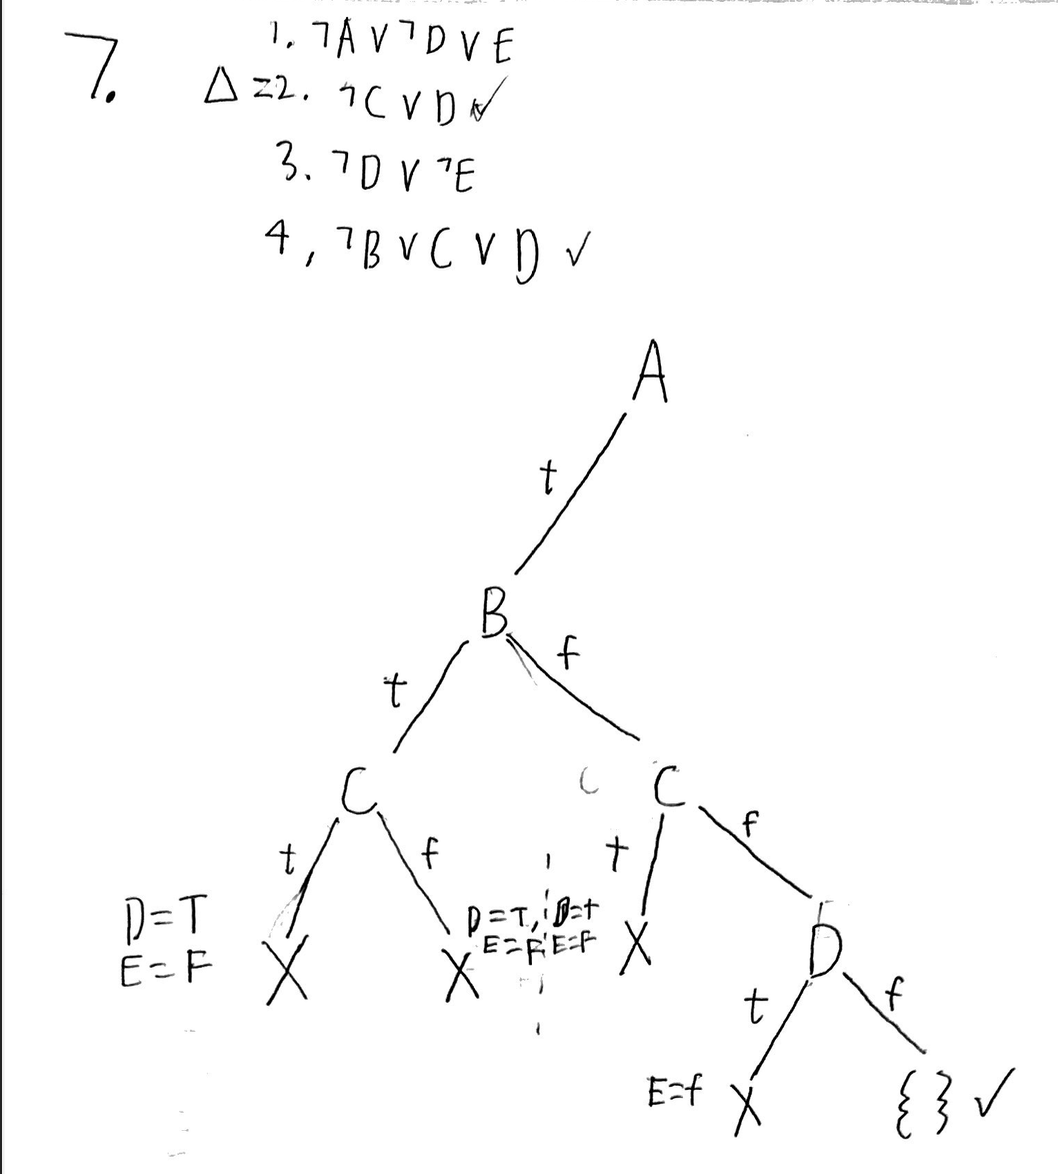
\includegraphics[width=0.4\textwidth]{src/q7.png}
\end{center}

\newpage
\question[12] Show the trace of DPLL+ on the above KB.

\begin{center}
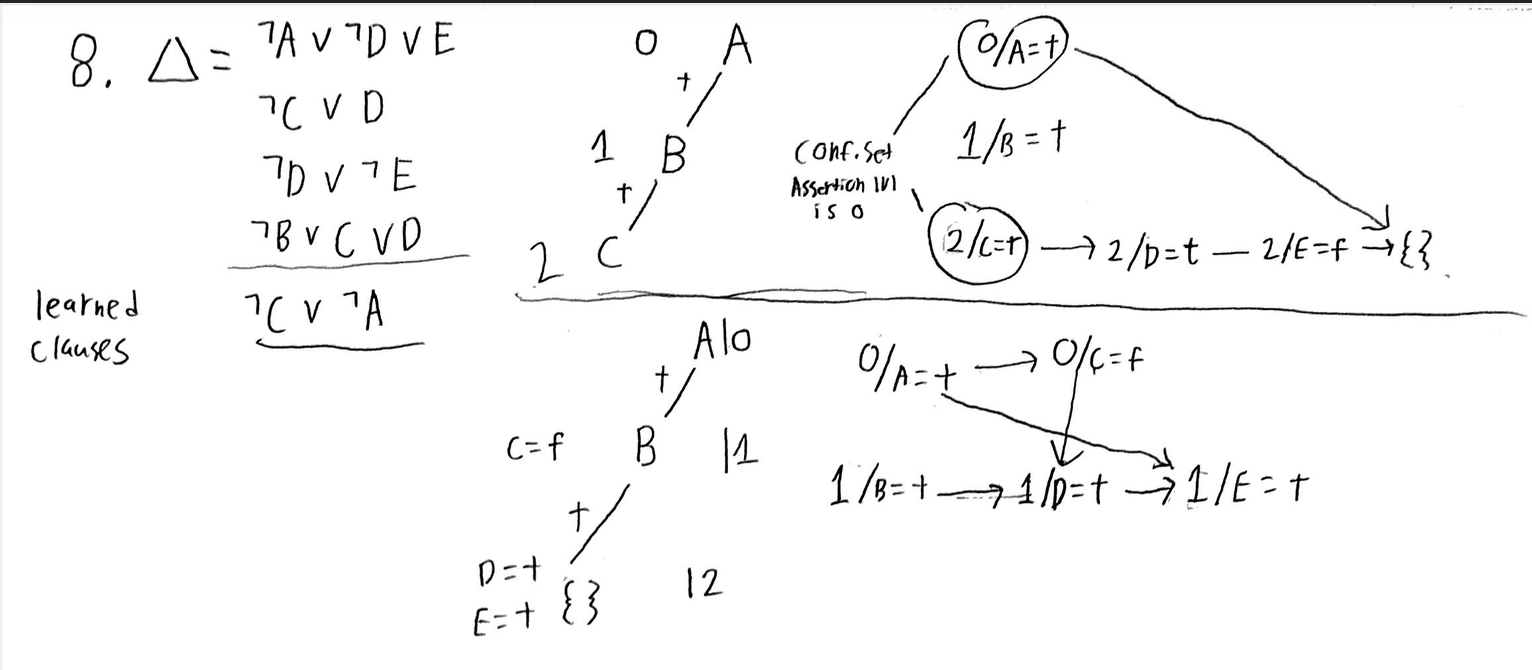
\includegraphics[width=0.8\textwidth]{src/q8.png}
\end{center}

\question[12] Consider the following knowledge base.
$$\Delta = A \Rightarrow B, \lnot A \Rightarrow (\lnot B \lor C), (B \lor D) \Rightarrow C$$
Show how you can count the number of models of $\Delta$ using CDPLL and draw the termination tree. Assume that you are expanding variables according to the order $A,B,C,D$ and always expand true before false.
\begin{center}
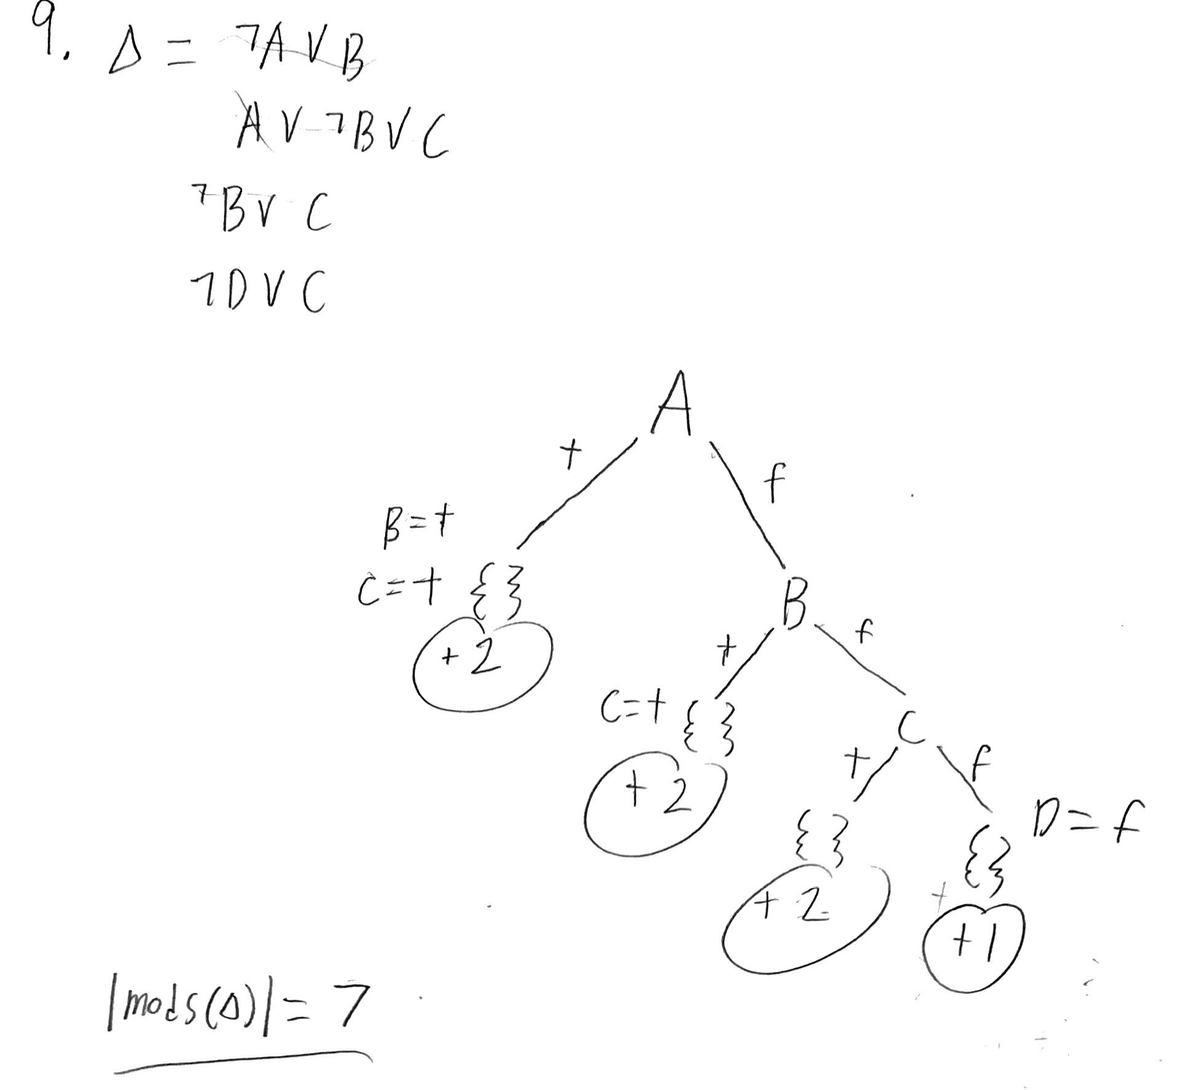
\includegraphics[width=0.8\textwidth]{src/q9.png}
\end{center}
\newpage

\question[14] Consisder the following knowledge base
$$\Delta = P_1 \lor P_2 \lor P_3, P_1 \Rightarrow Q, P_2 \Rightarrow Q, P_3 \Rightarrow Q$$
\begin{enumerate}[label={\alph*}]
    \item Convert $\Delta$ into clausal form.$$\Delta = P_1 \lor P_2 \lor P_3, \lnot P_1 \lor Q, \lnot P_2 \lor Q, \lnot P_3 \lor Q$$
    \item Apply directed resolution to the clausal form using the variable order $P_1,P_2,P_3,Q$
    \vspace{1em}

        % Table for directed resolution: variables, initial clauses, and new clauses
        \begin{center}
    \begin{tabular}{@{}p{1cm} p{5cm} p{7cm}@{}}
    	\textbf{Var} & \textbf{Initial clauses} & \textbf{New clauses} \\
    \hline
    $P_1$ & $\{\lnot P_1 \lor Q\},\ \{P_1 \lor P_2 \lor P_3\}$ & \\
    $P_2$ & $\{\lnot P_2 \lor Q\}$ & $\{P_2\lor P_3\lor Q\}$\\
    $P_3$ & $\{\lnot P_3 \lor Q\}$ & $\{P_3\lor Q\}$\\
    $Q$   &  & $\{Q\}$\\
    \end{tabular}
        \end{center}
\item Construct a decision tree for $\Delta$ and use it to count the number of models of $\Delta$.
\begin{center}
        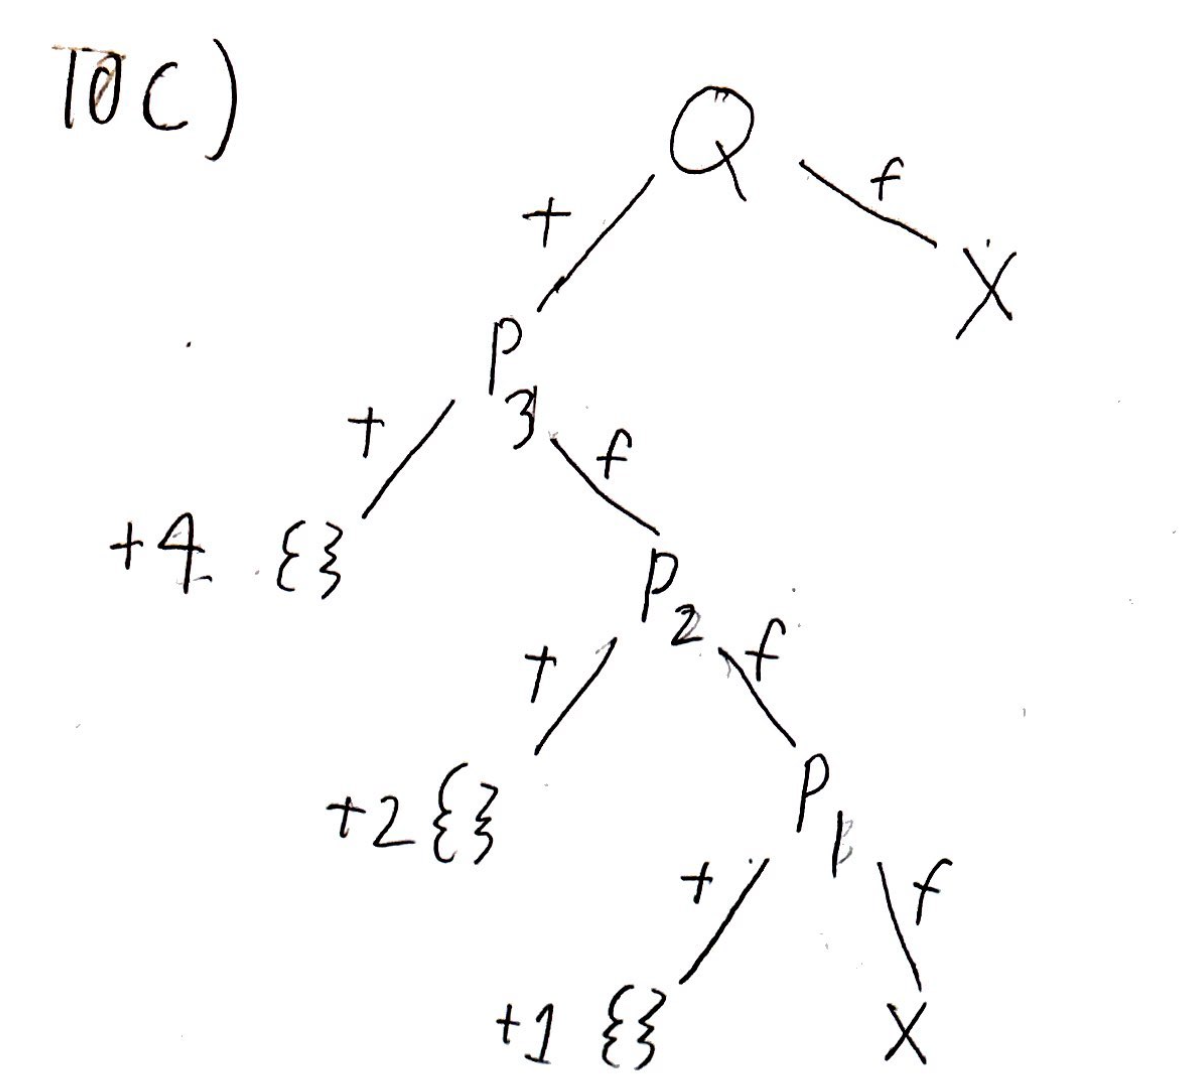
\includegraphics[width=0.4\textwidth]{src/q10.png}
    \end{center}
\end{enumerate}
\end{questions}

\end{document}
